% !TEX program = pdflatex
% PRL-format theory draft. Numerical details and audit tables are in suppl.tex.
\documentclass[aps,prl,reprint,superscriptaddress,nofootinbib]{revtex4-2}

\usepackage[T1]{fontenc}
\usepackage{lmodern}
\usepackage{microtype}
\usepackage{amsmath,amssymb,bm}
\usepackage{graphicx}
\usepackage[hidelinks]{hyperref}

\hypersetup{
  pdftitle={Double radiation cancellation at an acoustic Rayleigh threshold},
  pdfauthor={Author names to be inserted},
  pdfsubject={Theory of acoustic Rayleigh-threshold bound states in the continuum}
}

\newcommand{\ii}{\mathrm{i}}
\newcommand{\e}{\mathrm{e}}
\newcommand{\BIC}{\mathrm{BIC}}
\newcommand{\RA}{\mathrm{RA}}
\providecommand{\hom}{\mathrm{hom}}
\providecommand{\dr}{\mathrm{dr}}

\begin{document}

\title{Double Radiation Cancellation at an Acoustic Rayleigh Threshold}
\author{Author Name}
\affiliation{Affiliation to be inserted}
\author{Coauthor Name}
\affiliation{Affiliation to be inserted}
\date{\today}

\begin{abstract}
Bound states in the continuum require complete cancellation of radiation from
an eigenmode.  At a diffraction threshold, however, vanishing normal flux does
not imply confinement, because a finite grazing field remains nondecaying and
non-square-integrable.  We establish a strict Rayleigh-threshold bound state in
a periodic underwater acoustic surface.  The homogeneous state occurs exactly
when a first diffraction order opens, while both its threshold amplitude and
the amplitude of the remaining propagating order vanish.  A full outgoing-wave
operator, pole continuation, and exterior-norm saturation distinguish the
state from a Rayleigh anomaly and a high-$Q$ resonance.  Two groove-supported
source families independently cancel threshold and finite-flux radiation.
These results identify channel-opening BICs as a threshold subclass governed
by amplitude cancellation rather than zero flux alone.
\end{abstract}

\maketitle

A bound state in the continuum (BIC) is a spatially localized eigenstate at a
real frequency embedded in a radiation continuum.  Its defining property is
the complete disappearance of all outgoing components of a \emph{homogeneous}
mode, rather than a narrow feature in a driven spectrum
\cite{Hsu2016BIC,Koshelev2023Review,Azzam2021Review}.  Symmetry incompatibility,
Friedrich--Wintgen interference, Fabry--P\'erot trapping, and topological
radiation zeros provide established routes to this decoupling
\cite{Yang2014Analytical,Zhen2014Topological,Hsu2013Observation}.  These
mechanisms are normally formulated where the set of asymptotic radiation
channels remains fixed.

A diffraction threshold is qualitatively different.  When a Floquet order
reaches grazing propagation, its normal wavenumber and normal power flux
vanish, yet a finite pressure amplitude remains independent of the
surface-normal coordinate and is therefore not square-integrable.  Thus a
Rayleigh anomaly does not become a BIC merely because the grazing order carries
no normal power.  A strict threshold state must cancel the grazing amplitude
itself together with every other propagating amplitude.  This distinction
connects the square-root singularity of threshold scattering
\cite{Rayleigh1907,Wojcik2021ThresholdScattering} to the localization condition
for an embedded eigenstate.

Recent electromagnetic work describes a resonant pole reaching a Rayleigh
branch point \cite{Karavaev2026Rayleigh}, while acoustic BICs have been realized
through resonator interference, symmetry, and underwater Fabry--P\'erot
trapping \cite{Farhat2024UltrahighQ,Yang2024MergedFP}.  What remains unresolved
in scalar acoustic diffraction is whether a homogeneous mode can be localized
exactly as a new channel opens while another diffraction order is already
propagating.  We establish such a state in a periodic underwater acoustic
surface and test the threshold coefficient directly.

The state is formed by channel-resolved destructive interference.  Two
groove-supported source families acquire independent internal phases and close
separate radiation sums for the grazing and finite-flux channels.  A null of
the complete outgoing-wave operator, continuation of the associated pole, and
saturation of the exterior norm distinguish this state from both a generic
Rayleigh anomaly and a finite-linewidth resonance.  The result identifies
channel-opening BICs as a threshold subclass for which field-amplitude
cancellation, rather than zero flux alone, restores localization.

Consider a sound-hard surface of period $a$ occupying $y\leq0$, with water in
$y>0$ and time dependence $\e^{+\ii\omega t}$.  For incidence toward the
surface and outgoing reflection,
\begin{align}
 p_{\mathrm{inc}}&=\e^{-\ii k_{x,0}x+\ii k_{y,0}y},
 &p_{\mathrm{sc}}&=\sum_{n\in\mathbb Z}A_n^{\dr}
 \e^{-\ii k_{x,n}x-\ii k_{y,n}y},                                      \label{eq:fields}\\
 k_{x,n}&=k_0\sin\theta+\frac{2\pi n}{a},
 &k_{y,n}&=\sqrt{k_0^2-k_{x,n}^2}.                                      \label{eq:wavenumbers}
\end{align}
The outgoing branch has $\Re k_{y,n}\geq0$ and $\Im k_{y,n}\leq0$.  We use
\begin{equation}
 \Omega=\frac{af}{c},\qquad
 \kappa=\frac{ak_0\sin\theta}{2\pi}=\Omega\sin\theta,\qquad
 |\kappa+n|=\Omega                                                       \label{eq:rayleigh}
\end{equation}
for a Rayleigh threshold of order $n$.

The two-groove cell is shown in Fig.~\ref{fig:structure}; its complete
dimensional specification is given in the Supplemental Material.  At
$f=200$~kHz and $c=1500$~m/s,
\begin{align}
 \kappa_{\BIC}&=0.083848696553,\qquad
 \Omega_{\BIC}=0.916151303447,\nonumber\\
 \theta_{\BIC}&=\pm5.251216^{\circ}.                              \label{eq:point}
\end{align}
For $+\theta$, $n=0$ is propagating, $n=-1$ is at threshold because
$\kappa+\Omega=1$, and $n=+1$ is evanescent.  Reversing the Bloch number
exchanges $n=-1$ and $n=+1$.

\begin{figure*}[t]
  \centering
  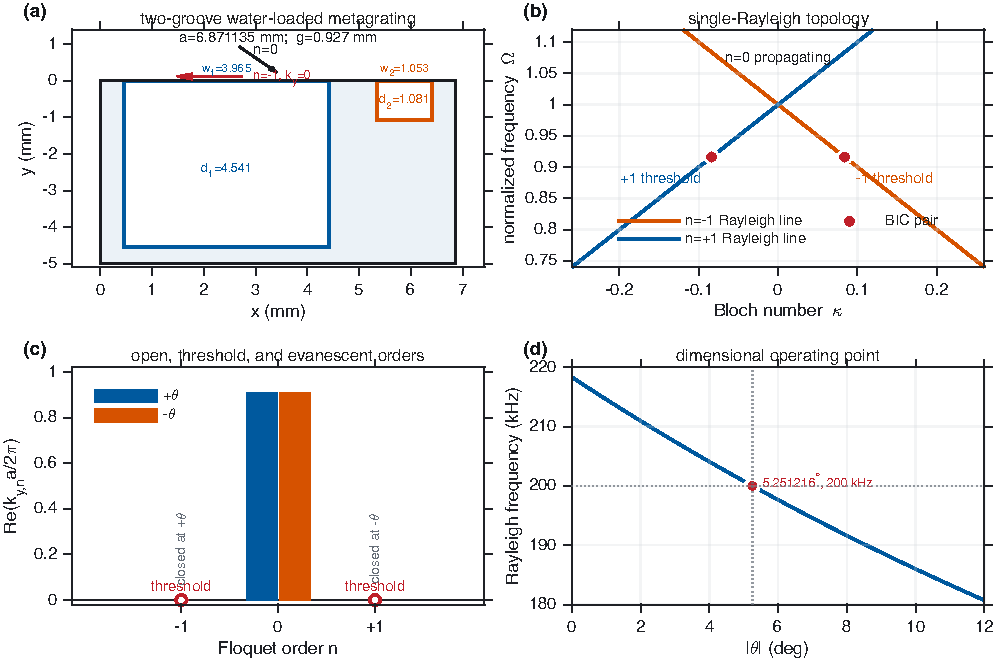
\includegraphics[width=\linewidth]{figures/fig1_structure_topology.pdf}
  \caption{\label{fig:structure}
  Acoustic realization and channel topology.  (a) Two-groove cell; dimensions are
  in millimeters.  (b) The two first-order Rayleigh lines and the reciprocal
  BIC pair.  The zeroth order is propagating at both points.  (c) Normal
  wavenumbers for the three displayed orders: for $+\theta$ ($-\theta$),
  $n=-1$ ($n=+1$) is grazing and the opposite first order is evanescent.
  (d) The positive-angle point on the dimensional $n=-1$ Rayleigh curve.}
\end{figure*}

\begin{figure*}[t]
  \centering
  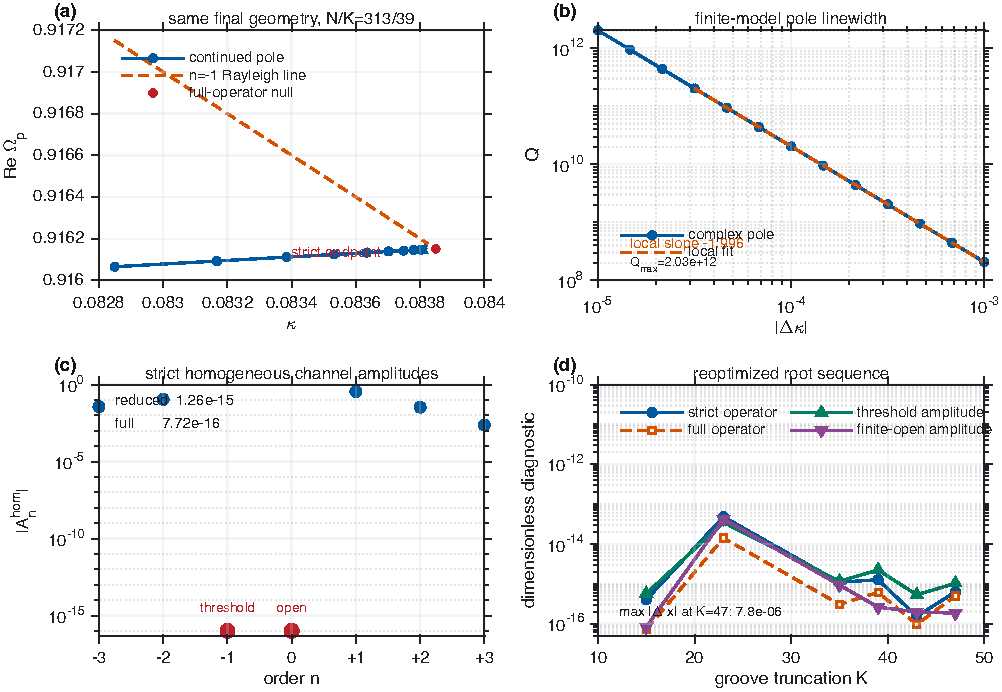
\includegraphics[width=\linewidth]{figures/fig2_strict_bic_evidence.pdf}
  \caption{\label{fig:evidence}
  Strict-null evidence.  (a) Final-geometry pole trajectory and the
  $n=-1$ Rayleigh line.  The red endpoint is also a null of the full
  $(313,39)$ operator.  (b) Pole quality factor and local fit; the exponent
  is a resolved finite-model trend.  (c) Final homogeneous Floquet
  amplitudes.  The finite-flux $n=0$ and threshold $n=-1$ coefficients
  vanish, while the displayed remaining orders are evanescent.
  (d) Reoptimized root sequence: reduced and full singular-value ratios and
  the independently extracted threshold/open amplitudes remain at machine
  precision through $(377,47)$.}
\end{figure*}

\begin{figure*}[t]
  \centering
  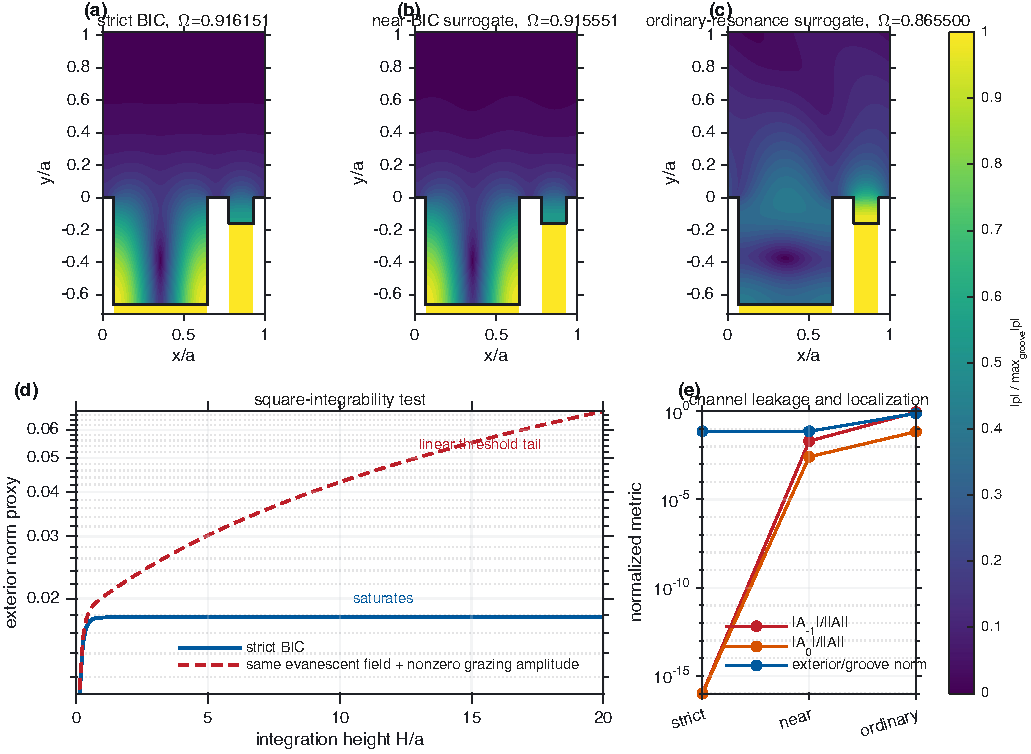
\includegraphics[width=\linewidth]{figures/fig3_homogeneous_fields.pdf}
  \caption{\label{fig:fields}
  Homogeneous pressure fields and localization.  (a) Strict BIC.
  (b) Near-BIC real-axis surrogate at $\Omega=0.9155513$.
  (c) Ordinary-resonance real-axis surrogate at $\Omega=0.8655$.
  All maps show $|p|/\max_{\mathrm{groove}}|p|$ on the same scale; white
  regions are rigid material.  (d) Exterior norm versus integration height
  for the strict mode and for the same evanescent field with a nonzero
  grazing component added.  (e) Threshold amplitude, finite-open amplitude,
  and exterior-to-groove norm proxies.  Panels (b,c) are diagnostic
  surrogates, not exact quasinormal-mode fields.}
\end{figure*}

\begin{figure*}[t]
  \centering
  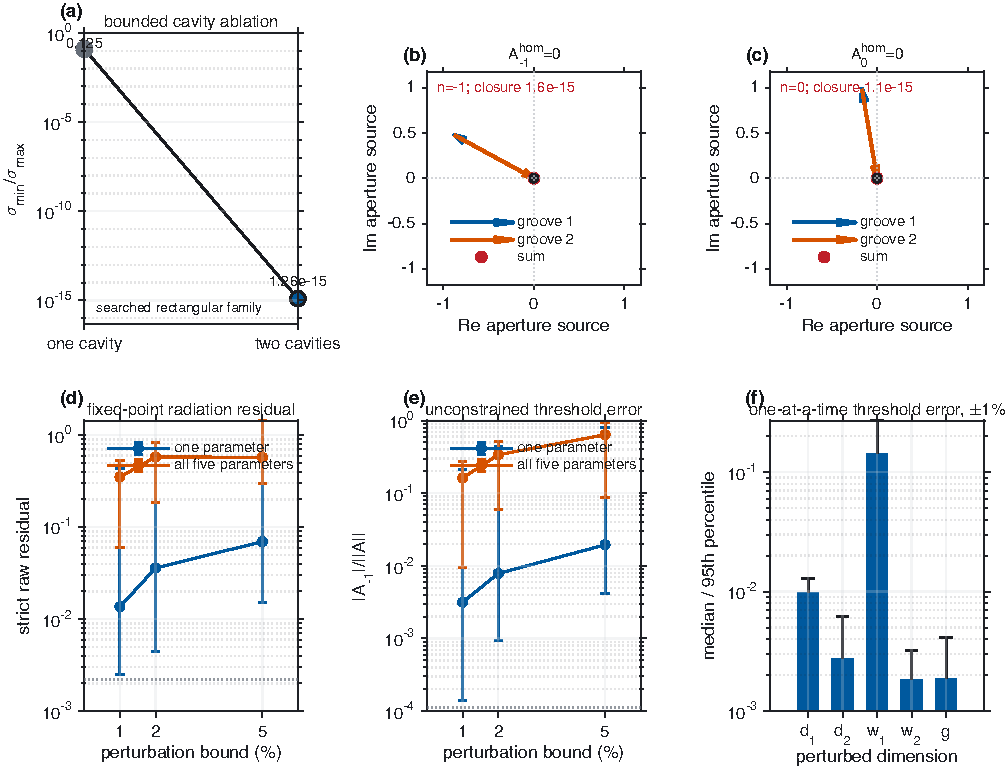
\includegraphics[width=\linewidth]{figures/fig4_dof_tolerance.pdf}
  \caption{\label{fig:mechanism}
  Cavity degrees of freedom and fixed-point sensitivity.
  (a) Best single-large-cavity result in the searched rectangular family
  versus the two-groove root.  (b,c) Separate aperture-source phasor closures
  for the grazing $n=-1$ and propagating $n=0$ constraints.
  (d,e) Medians and 5--95\% intervals of the strict raw residual and the
  unconstrained threshold-amplitude error for one-parameter and joint
  perturbations.  The dotted line is the unperturbed $(185,23)$ numerical
  floor.  (f) One-at-a-time $\pm1\%$ sensitivity; bars are medians and
  whiskers are 95th percentiles.}
\end{figure*}

Inside groove $\ell$, a bottom-rigid cosine expansion is retained.  Projecting
pressure and normal-velocity continuity without eliminating the groove
coefficients gives the pole-free homogeneous system
\begin{equation}
 \mathsf F(\omega,\kappa;\bm g)
 \begin{bmatrix}\bm A^{\hom}\\ \bm C\end{bmatrix}=0,
 \qquad \bm g=(d_1,d_2,w_1,w_2,g).                                      \label{eq:operator}
\end{equation}
The full block matrix, scaling, and driven reduction are given in the
Supplemental Material.  This separation is essential: $A_n^{\dr}$ contains
the forced background response, whereas $A_n^{\hom}$ belongs to an outgoing
eigenmode.

For a single homogeneous exterior order, define the height-integrated
pressure norm $\mathcal N_n(H)$ by
\begin{equation}
 \mathcal N_n(H)=\int_0^H |p_n^{\hom}|^2\,\mathrm{d}y.
 \label{eq:norm-definition}
\end{equation}
It evaluates to
\begin{equation}
 \mathcal N_n(H)=
 \begin{cases}
 H|A_n^{\hom}|^2,&k_{y,n}=0,\\[2pt]
 \dfrac{|A_n^{\hom}|^2}{2\alpha_n}
 (1-\e^{-2\alpha_nH}),&k_{y,n}=-\ii\alpha_n.
 \end{cases}                                                            \label{eq:norm}
\end{equation}
Thus the positive-angle state is strict only if
\begin{equation}
 A_{-1}^{\hom}=0,\qquad A_0^{\hom}=0.                                   \label{eq:strict}
\end{equation}
We first impose Eq.~\eqref{eq:strict} by removing those two amplitude columns
from the unknown vector, row- and column-scale the remaining operator, and
reconstruct its smallest right singular vector.  At $(N,K)=(313,39)$,
where $N$ is the number of exterior orders and $K$ is the cosine-mode count
per groove,
\begin{align}
 \sigma_{\min}/\sigma_{\max}&=1.2603643\times10^{-15},\nonumber\\
 r_{\mathrm{raw}}&=1.3765668\times10^{-13}.                         \label{eq:residual}
\end{align}
This constrained null is not the sole evidence.  Evaluating the complete
complex-frequency operator at the same final geometry, with the selected
$k_{y,-1}$ set exactly to zero, gives
$\sigma_{\min}/\sigma_{\max}=7.7151\times10^{-16}$ and an unconstrained null
whose open and threshold amplitudes vanish at machine precision.

The null persists under modal refinement, and a same-geometry complex-pole
continuation remains on one branch while approaching the real Rayleigh
endpoint [Fig.~\ref{fig:evidence}].  These tests support a converging embedded
eigenstate rather than a real-axis minimum generated by the threshold
singularity.  The truncation sequence, mode overlaps, quality factors, and
finite-model scaling fit are reported in the Supplemental Material.

Figure~\ref{fig:fields} provides a spatial test.  The strict mode contains only
evanescent exterior orders, and its exterior norm saturates within a few
periods.  Restoring any nonzero grazing amplitude produces the linear term in
Eq.~\eqref{eq:norm}.  Near-BIC and ordinary-resonance real-axis surrogates are
shown only as discriminating controls; their reconstruction and channel errors
are detailed in the Supplemental Material.

The two zero conditions can be resolved into aperture-source phasors,
\begin{equation}
 A_m^{\hom}=\sum_{\ell=1}^{2}\sum_q
 \mathcal R_{m,\ell q}C_{\ell q}=0,
 \qquad m\in\{-1,0\}.                                                    \label{eq:phasor}
\end{equation}
The two grooves close the $n=-1$ and $n=0$ phasor polygons separately, with
normalized closure errors $1.6\times10^{-15}$ and $1.1\times10^{-15}$.
This motivates, but does not prove universally, the need for two independent
phase controls.  A global search over a \emph{single large rectangular}
groove, retaining transverse modes and varying
$0.04\leq\kappa\leq0.25$, $0.04\leq d/a\leq2$, and
$0.50\leq w/a\leq0.95$, reaches only
$\sigma_{\min}/\sigma_{\max}=0.124588$ at $(221,44)$.  The comparison is
therefore a bounded ablation within this declared shape family, not a no-go
theorem for arbitrary one-cavity structures.

Fabrication perturbations, dimensional similarity, sound-speed detuning, and
driven scattering are reported in the Supplemental Material.  They delimit
the ideal eigenstate result but are not used to certify it.  In particular,
the driven response is not interpreted as a converged one-way device, and a
separate high-efficiency off-Rayleigh point is an ordinary anomalous reflector
rather than a BIC signature.

We have established a strict acoustic bound state at a Rayleigh channel
opening.  Localization requires cancellation of both the zero-flux threshold
amplitude and the coexisting finite-flux radiation amplitude.  The two-groove
realization exposes these conditions as separate interference constraints,
identifying channel-opening BICs as a threshold subclass of embedded
eigenstates.  The result applies to an infinite, rigid, lossless acoustic
surface; finite-size leakage, dissipation, elastic compliance, and experimental
realization remain outside the present claim.

\clearpage
\bibliography{ref}

\end{document}
